\onecolumn
\icmltitle{Supplementary material}
\appendix








\section{Non-connected data manifolds and intersections}
\label{sec:non-connected}

Earlier we assumed that the data comes from a connected manifold $M$, whose local dimension is constant. Moreover, it was embedded in $\R^D$, precluding self-intersections. These restrictions can be relaxed as follows. Firstly, we may allow $M$ to contain multiple connected components. Secondly, instead of an embedding, we may consider a \emph{good} immersion $j\colon M\to \R^D$, satisfying the following finiteness condition.

\begin{definition}
\label{def:good-immersion}
    We will call an immersion $j\colon M\to N$ \emph{good}, if $M$ admits an open cover $\C$ such that for every $U\in\C$ the restriction of $j$ to $U$ is an embedding, and moreover, every $x\in N$ has an open neighborhood whose preimage intersects only finitely many sets in $\C$.
\end{definition}

In the non-connected case, the dimension is no longer constant on the manifold, but can differ between its components. We will denote by $\dim_x M$ the dimension of $M$ at a point $x\in M$.

Before we proceed, we will prove a simple technical lemma.

\begin{lemma}
\label{lem:finite-component-intersection}
    Let $j\colon M\to N$ be a good immersion. Then every $x\in N$ has a neighborhood whose preimage intersects only finitely many connected components of $M$.
\end{lemma}

\begin{proof}
    Let $\C$ be an open cover of $M$ satisfying conditions of Definition~\ref{def:good-immersion}. Take $x\in N$, and let $V \subset N$ be a neighborhood of $x$ such that $j^{-1}(V)$ intersects only finitely many sets $U_1,\dots, U_n\in\C$. On each $U_i$ the restriction of $j$ is an embedding, so there exists a neighborhood $V_i\subset V$ of $x$ whose preimage is contained in a single connected component of $U_i$, and hence in a single connected component $M_i$ of $M$. 
    
    The intersection $\bigcap_i V_i$ is the required neighborhood of $x$, as its preimage is contained in the finite union of connected components $\bigcup_i M_i$.
\end{proof}

This more general case reduces to the one studied in Section~\ref{sec:core-estimate}, as the following reasoning shows.

\begin{proposition}
\label{prop:resolution-of-intersections}
    Suppose $j\colon M\to N$ is an immersion of manifolds. Moreover, let $\mu$ be a smooth measure on $M$. Then there exists a manifold $\tilde{M}$ endowed with a measure $\tilde{\mu}$ and a local diffeomorphism $f\colon\tilde{M}\to M$, such that 
    \begin{enumerate}
        \item the measure $\tilde{\mu}$ is smooth
        \item the pushforward $f_*\tilde{\mu}$ equals $\mu$;
        \item $\tilde\jmath = j\circ f\colon \tilde{M}\to N$ restricted to every connected component of $\tilde{M}$ is an embedding.
        \item if $j$ is good, then so is $\tilde\jmath$;

    \end{enumerate}    
\end{proposition}

\begin{proof}
    Since $j$ is an immersion, there exists an open cover $\C$ of $M$ such that on every $U\in\C$ the restriction of $j$ is an embedding. Let $\{\psi_U : U\in\C\}$ be a partition of unity subordinate to $\C$. Denote $M_U = \{x\in M : \phi_U(x) > 0\}$, and let $f_U\colon M_U\to M$ be the corresponding inclusion map. Finally, let $\tilde{M}$ be the disjoint union of $\{M_U : U\in\C\}$, and define $f\colon \tilde{M}\to M$ by gluing together the inclusions $f_U$.
    
    The measure $\tilde{\mu}$ can be defined as
    \begin{equation}
        \tilde{\mu} = \sum_{U\in\C} (f_U^{-1})_*(\psi_U \mu),
    \end{equation}
    i.e.\ for every $U\in\C$ we multiply $\mu$ by density function $\psi_U$, restrict it to $M_U$ and pull it to $\tilde{M}$ through $f_U$. Since by definition $\psi_U$ is continuous and positive on $M_U$, the measure $\tilde{\mu}$ is smooth. Moreover, by construction we have $f_*\tilde{\mu} = \mu$,     and the restriction of $\tilde\jmath$ to every $M_U$ (and therefore every to every connected component) is an embedding.

    To show the last assertion, assume that $j$ is good. In this case, the cover $\C$ defined above can be chosen in such a way that for every $x\in N$ there exists a neighborhood $V\subset N$ whose preimage $j^{-1}(V)$ intersects only finitely many sets in $\C$. It is then easy to see that the cover $\{M_U : U\in\C\}$ of $\tilde{M}$ satisfies the conditions of Definition~\ref{def:good-immersion}, so $\tilde\jmath$ is good.
\end{proof}

Now, suppose that in Theorem~\ref{thm:core-estimate}, instead of an embedded submanifold $S$, we are dealing with the image of a proper immersion $j\colon M\to \R^D$, and that $p_S$ is the pushforward of a probability measure $\mu$ on $M$. Thanks to Proposition~\ref{prop:resolution-of-intersections}, this reduces to the situation where $j$ restricted to every connected component of $M$ is an embedding.

\begin{proposition}
    Suppose $j\colon M\to \R^D$ is a good immersion, and its restriction to every connected component of $M$ is an embedding. Let $\mu$ be a smooth probability measure on $M$, and $p_S=j_*\mu$. For $x\in S = j(M)$ and sufficiently small $\delta$ we have
    \begin{equation}
        \log\rho_\delta(x) = (d-D)\log\delta + O(1),
    \end{equation}
    where 
    \begin{equation}
        d = \min_{j(y)=x} \dim_y M.
    \end{equation}
\end{proposition}

\begin{proof}
    By Lemma~\ref{lem:finite-component-intersection}, for sufficiently small $r$ the preimage $j^{-1}(B)$ of the ball $B=B(x,r)$ centered at $x$ intersects only finitely many connected components of $M$. Denote them by $M_1,\dots, M_k$, and let $M_0$ be the union of the remaining components. The measure $\mu$ can be decomposed as
    \begin{equation}
        \mu = \sum_{i=0}^k \mu(M_i)\mu_i,
    \end{equation}
    where $\mu_i$ is the restriction of $\mu$ to $M_i$, normalized to a probability measure. If we put $p_i = j_*\mu_i$, a similar decomposition holds for $p_S$.
    
    If we apply Theorem~\ref{thm:core-estimate} to $j(M_i)$ endowed with the measure $p_i$, for $i>0$, the corresponding perturbed density $\rho^i_\delta$ satisfies
    \begin{equation}
        \rho^i_\delta(x) \asymp \delta^{\dim{M_i}-D}
    \end{equation}
    for sufficiently small $\delta$. Moreover, for $\delta < r^2$, we have $j(M_0) = j(M_0)\setminus B(x,\delta^{1/2})$, so by Lemma~\ref{lem:gaussian-estimate-outside-ball}
    \begin{equation}
        \lim_{\delta\to 0^+} \rho^0_\delta(x) = 0.
    \end{equation}
    Consequently, for small $\delta<1$
    \begin{equation}
        \rho_\delta(x) = \sum_{i=0}^k \mu(M_i)\rho^i_\delta(x) \asymp \sum_{i=1}^k \delta^{\dim{M_i}-D},
    \end{equation}
    and the term with the lowest exponent dominates.
\end{proof}
  
  
\section{Examples with explicit derivations}

\subsection{A motivating example}
\label{sec:motivating-example}

Consider the standard embedding $\R^d \subset \R^D$. Take for $S$ a bounded open subset of $\R^d$, endowed with the uniform probability measure $p_S$ with constant density $\rho\equiv\operatorname{vol}(S)^{-1}$ on $S$. If we denote by $x_1$ and $x_2$ the components of a vector $x\in \R^D$ corresponding to the standard decomposition $\R^D = \R^d \times \R^{D-d}$, it follows from \eqref{eq:mollified-density} and properties of the Gaussian function, that
\begin{equation}
    \label{eq:flat-example-mollified-density}
    \rho_\delta(x) = 
    \frac{\phi^{D-d}_{\delta}(x_2)}{\operatorname{vol}(S)} 
    \int_S \phi^d_{\delta}(x_1-y_1) \, d y_1.
\end{equation}

Now, if $x$ is an interior point of $S$, then $x_2=0$. Moreover, for sufficiently small $\delta$, the integral above is arbitrarily close to $1$, as most of the mass of the integrand falls into a small neighborhood of $x_1$, which is contained in $S$. Therefore, for sufficiently small $\delta$
\begin{equation}
    \rho_\delta(x) \asymp \phi^{D-d}_\delta(0) = \delta^{d-D}\phi^{D-d}(0) \asymp \delta^{d-D}
\end{equation}
uniformly in $\delta$.

It follows that
\begin{equation}
    \log \rho_\delta(x) = (d-D) \log\delta + O(1),
\end{equation}
and hence
\begin{equation}
    d-D = \lim_{\delta\to 0} \frac{\log \rho_\delta(x)}{\log\delta}.
\end{equation}
In practice, $d-D$, and in consequence $d$, can be estimated by considering $\rho_\delta(x)$ for multiple small values of $\delta$, and using linear regression. 



\subsection{Normal distribution in $\R^D$}
\label{sec:delta-gaussian-dimensions}
Suppose that $S=\R^D$, and $p_S = \N(0, \Sigma)$, where $\Sigma$ is a diagonal matrix with entries $\sigma_1^2 \geq \sigma_2^2 \geq\dots\geq \sigma_D^2$. In this case, the perturbation with $\N(0, \delta^2 I)$ yields another normal distribution $\N(0, \Sigma + \delta^2 I)$, whose density at $0$ is
\begin{equation}
\label{eq:perturbed-normal-distribution-at-0}
    \rho_\delta(0) = (2\pi)^{-D/2}\prod_{k=1}^D (\sigma_k^2 + \delta^2)^{-1/2}.
\end{equation}

\begin{proposition}
    \label{prop:delta-gaussian-dimensions}
    Let $1 \leq d < D$, and denote $\tau = (\sigma_d\sigma_{d+1})^{1/2}$. For $\lambda \geq 1$ and $\delta\in [\lambda^{-1}\tau, \lambda\tau]$ we have
    \begin{equation}
        \log\rho_\delta(0) = (d-D)\log\delta + M - C_\lambda,
    \end{equation}
    where $M$ is independent of $\delta$, and  $0 \leq C_\lambda \leq \frac{D\sigma_{d+1}}{2\sigma_d} \lambda^2$.
\end{proposition}
In other words, the above proposition states that for $\delta$ between two consecutive deviations $\sigma_d$ and $\sigma_{d+1}$, our LID estimate is approximately the number $d$ of dimensions in which the Gaussian distribution is `thicker' than $\delta$, and the approximation error decreases with the growth of the ratio $\sigma_d/\sigma_{d+1}$ and the distance of $\delta$ from $\sigma_d$ and $\sigma_{d+1}$.

\begin{proof}
    Let us denote $\eta = \lambda(\sigma_{d+1}/\sigma_d)^{1/2}$. The, for $k\leq d$ we may compute $\lambda\tau = \eta\sigma_d \leq \eta\sigma_k$, which leads to 
    \begin{equation}
        \sigma_k^2 + \delta^2
        \leq  (1 + \eta^2)\sigma_k^2.
    \end{equation}
    On the other hand, for $k \geq d+1$, we have $\lambda^{-1}\tau = \eta^{-1}\sigma_{d+1} \geq \eta^{-1}\sigma_k$, and similarly to the previous case, we have
    \begin{equation}
        \sigma_k^2 + \delta^2
        \leq 
        (1+\eta^2)\delta^2.
    \end{equation}
    By applying these two estimates to the formula~\eqref{eq:perturbed-normal-distribution-at-0} for $\rho_\delta(0)$ we are able to obtain a two-sided estimate
    \begin{equation}
        M(1+\eta^2)^{-D/2} \delta^{d-D}
        \leq \rho_\delta(0) 
        \leq M\delta^{d-D}, 
    \end{equation}
    with $M=(2\pi)^{-D/2} \prod_{k=1}^d \sigma_k^{-1}$ independent of $\delta$. Finally, after taking $\log$ we can see that
    \begin{equation}
        \log \rho_\delta(0) = (d-D)\log\delta + \log M - \frac{D}{2}\log(1+\eta^2),
    \end{equation}
    and the last term is positive and bounded from above by $D\eta^2/2$, yielding the desired estimate by substituting $\eta$.
\end{proof}

From the above Proposition we can see that if there is a large gap between $\sigma_d$ and $\sigma_{d+1}$, then for $\delta$ in the neighborhood of their geometric mean, the LID estimate obtained through linear regression should be approximately $d$, with approximation error decreasing, and the range of viable $\delta$ increasing with the growth of the gap size, expressed by the ratio $\sigma_{d+1}/\sigma_d$.


\subsection{Points along a line}

Consider a zero-dimensional manifold $M$, consisting of $N$ points, endowed with uniform probability measure. Suppose $M$ is embedded into $\R^D$ in such a way that its image $\set{x_1, \dots, x_N}$ is actually contained in $\R \subset \R^D$, and has the form $x_k = (\xi_k, 0, \dots, 0)$, where $\xi_{k+1} \geq \xi_k + \eta$ for some $\eta > 0$, i.e.\ the indexing is chosen in such a way that the points $x_k$ are ordered along $\R$, and the distances between them are at least $\eta$.

In this setting, we will study the quantity $\rho_\delta(x_n)$ more closely, and attempt to understand its relationship with the perturbation magnitude for any $\delta$, not just sufficiently small ones. We have
\begin{equation}
    \rho_\delta(x_0) 
    = \frac{1}{N}\sum_{k=1}^N \phi^D_\delta(x_n-x_k) 
    = \frac{\phi^D_\delta(0)}{N} \Bigg( 1 + \sum_{\substack{k =1\\ k\ne n}}^N \frac{\phi^D_\delta(x_n-x_k) }{\phi^D_\delta(0)} \Bigg)
    = M \delta^{-D} \left( 1 + \epsilon_\delta\right),
\end{equation}
where $M=({N(2\pi)^{D/2}})^{-1}$, and
\begin{equation}
    \epsilon_\delta 
    = \sum_{\substack{k =1\\ k\ne n}}^N \frac{\phi^D_\delta(x_n-x_k)}{\phi^D_\delta(0)}
    = \sum_{\substack{k =1\\ k\ne n}}^N \exp \left[ -\frac{1}{2} \left(\frac{\xi_n-\xi_k}{\delta}\right)^2\right].
\end{equation}

After taking $\log$, we get
\begin{equation}
    \log \rho_\delta(x_0) = -D\log\delta + \log M + \log(1+ \epsilon_\delta),
\end{equation}
where the term $\log M$ is independent of $\delta$, and $0 \leq \log(1+\epsilon_\delta) \leq \epsilon_\delta$.

\begin{proposition}
\label{prop:points-along-line-upper-bound}
    Let $\lambda \geq 1$. If $\delta < \eta / (\sqrt{2}\lambda)$ then $\epsilon_\delta \leq 4e^{-\lambda^2}$.  In particular, for $\epsilon > 0$, we have $\epsilon_\delta < \epsilon$ provided that 
    \begin{equation}
        \delta < \frac{\eta}{(-2\log(\epsilon/4))^{1/2}},
    \end{equation}
    i.e.\ the threshold value for $\delta$ depends logarithmically on $\epsilon$.
\end{proposition}
\begin{proof}
    We have $\abs{\xi_i - \xi_j} \geq \eta\abs{i-j}$, and therefore
    \begin{equation}
        \epsilon_\delta \leq \sum_{\substack{k =1\\ k\ne n}}^N \exp \left[ -\frac{1}{2} \left(\frac{\eta(n-k)}{\delta}\right)^2\right]
        \leq \sum_{\substack{k =1\\ k\ne n}}^N e^ {-{\lambda^2} (n-k)^2}.
    \end{equation}
    For an upper estimate, we may also extend the summation over all integers except $n$, obtaining 
    \begin{equation}
        \epsilon_\delta 
        \leq \sum_{k\ne n} e^ {-{\lambda^2} (n-k)^2}
        = 2\sum_{j=1}^\infty e^ {-{\lambda^2} j^2}
        \leq 2\sum_{j=1}^\infty e^ {-{\lambda^2} j}
        = \frac{2}{1-e^{-\lambda^2}} e^{-\lambda^2}.
    \end{equation}
    For $\lambda \geq 1$ we have $(1-e^{-\lambda^2})^{-1} \leq 2$, so in the end $\epsilon_\delta \leq 4e^{-\lambda^2}$. By solving $\epsilon = 4e^{-\lambda^2}$ for $\lambda$ we obtain $\lambda = (-\log(\epsilon/4))^{1/2}$, yielding the last assertion.
\end{proof}




































\section{Ideal LIDL for normal distribution on a line}
\label{sec:appendix-lidl-for-normal-distribution}

Suppose our submanifold $S$ is the image of the standard embedding $\R\subset\R^D$, and let $p_S=\N(0,1)$. In this case, the perturbed distribution is $\N(0,\Sigma)$, where $\Sigma$ is a diagonal matrix with entries $(1+\delta^2, \delta^2, \dots, \delta^2)$. The density $\rho_\delta$ at a point $x=(t,0,\dots,0)\in S$ is therefore
\begin{equation}
    \rho_\delta(x) =  \frac{\delta^{1-D}}{(2\pi)^{D/2}(1+\delta^2)^{1/2}} \exp\left( -\frac{t^2}{2(1+\delta^2)}\right),
\end{equation}
and its logarithm can be decomposed into the following sum
\begin{equation}
    \log\rho_\delta(x) = 
        (1-D)\log\delta 
        - \frac{D}{2}\log(2\pi)
        - \frac{1}{2}\log(1+\delta^2)
        - \frac{t^2}{2(1+\delta^2)}.
\end{equation}
Let us now apply the trivial case of linear regression involving only two points, amounting to computing the slope of the line passing through two points. We have
\begin{equation}
    \frac{\log\rho_{\delta_1}(x) - \log\rho_{\delta_2}(x)}{\log\delta_1 - \log\delta_2} = 
        1 - D - \epsilon(t)
        ,
\end{equation}
where the error term expands to
\begin{equation}
    \epsilon(t)= \frac{1}{2(\log\delta_1 - \log\delta_2)}
            \left[ \log\frac{1+\delta_1^2}{1+\delta_2^2}
            - t^2 \left( \frac{1}{1+\delta_1^2} - \frac{1}{1+\delta_2^2} \right)\right],
\end{equation}
yielding a LID estimate $\hat{d}_x = 1 - \epsilon(t)$ at $x$.
We can see that the error $\epsilon$ decomposes into two terms of opposite signs. The first term depends only on $\delta$, and the second one, grows quadratically with $t$.

If we put $\delta_1=\eta\delta$, and $\delta_2=\delta$, the coefficient of $t^2$ can be further rewritten as
\begin{equation}
    \frac{1}{2(\log\delta_1 - \log\delta_2)} \left( \frac{1}{1+\delta_1^2} - \frac{1}{1+\delta_2^2} \right) 
    = \frac{\delta^2(1-\eta^2)}{2\log\eta(1+\delta^2)(1+(\delta\eta)^2)} \asymp \frac{\delta^2(1-\eta^2)}{2\log\eta},
\end{equation}
where the estimate holds uniformly in $\delta$ if $\delta$ is bounded $\delta$ from above. Although for fixed $\delta$ and $\eta$ the error is unbounded as a function of $t$, if we were allowed to adjust $\delta$ based on $t$ (with fixed $\eta$), for the error $\epsilon(t)$ to be bounded in $t$ it is necessary and sufficient that $\delta \leq C/t$ for some constant $C$.

Finally, the expected error for the LID estimate (computed in the above manner) at a random $x$ drawn from our distribution can be computed
\begin{equation}
\begin{split}
    \int_\R \epsilon(t)\phi^1(t) \,dt 
    & = \frac{1}{2(\log\delta_1 - \log\delta_2)}
            \left[ \log\frac{1+\delta_1^2}{1+\delta_2^2}
            - \int_\R t^2 \phi^1(t) \,dt\left( \frac{1}{1+\delta_1^2} - \frac{1}{1+\delta_2^2} \right)\right] = \\
    & = \frac{1}{2(\log\delta_1 - \log\delta_2)}
            \left[ \log\frac{1+\delta_1^2}{1+\delta_2^2}
            - \left( \frac{1}{1+\delta_1^2} - \frac{1}{1+\delta_2^2} \right)\right] 
    = \epsilon(1),
\end{split}
\end{equation}
where the last integral is just the variance of $\N(0,1)$, i.e.\ $1$.

\section{Normalizing Flows}
\label{sec:nf}

NF are very flexible tools for approximating probability distributions. They use parametrized nonlinear invertible transformation $f_\theta$ and change of variable formula to transform a simple density $\pi(z)$ into a more complicated one. NF are trained using gradient-based methods (e.g. SGD) to maximize log-likelihood of the data
$$\max_\theta \sum_{i}\log q(x_i)$$
where
$$q(x) = \pi(f_\theta(x))\left|\det\frac{\partial f_\theta(x)}{\partial x}\right|.$$
We used MAF \citep{papamakarios2017masked}, RQ-NSF \citep{durkan2019neural} and Glow \citep{kingma2018glow} models in our experiments. More detailed introduction to normalizing flows can be found in \cite{dinh2014nice}.


\begin{table}[h!]
\centering
\captionof{table}{Relative bias of LID estimates. All algorithm names explained in Table~\ref{tab:skdim}}\label{tab:comparison}
\scalebox{0.88}{
\begin{tabular}{ | c | c || c | c || c | c | c | c | c |  c | c | c | c | c |}
 \hline
 Distribution & LID &LIDL$_{M}$&LIDL$_{R}$&COR&ESS&KNN&LPC& MAD&MIN&MLE&MOM&TLE&TWO \\ \hline\hline


Lollipop in $\R^2$&0&\textbf{0.00}&\textbf{0.00}&1.67&1.67&1.60&1.67&1.82&1.67&1.80&1.74&-&1.65\\\hline
Lollipop in $\R^2$&1&\textbf{0.00}&\textbf{0.01}&\textbf{0.00}&\textbf{0.00}&0.58&\textbf{0.01}&0.10&\textbf{0.00}&\textbf{0.05}&\textbf{0.00}&-&\textbf{0.00}\\\hline
Lollipop in $\R^2$&2&\textbf{-0.00}&\textbf{-0.00}&\textbf{-0.01}&\textbf{-0.00}&-0.07&\textbf{0.00}&0.10&\textbf{-0.00}&0.08&\textbf{0.01}&-&\textbf{-0.03}\\\hline
$\U$ on helix in $\R^3$&1&\textbf{0.01}&\textbf{0.00}&\textbf{0.00}&\textbf{0.00}&0.68&\textbf{0.00}&0.12&\textbf{0.00}&0.06&\textbf{0.00}&\textbf{0.00}&\textbf{0.00}\\\hline
$\U$ on $S^7 \subseteq \R^8$&7&\textbf{-0.00}&\textbf{0.00}&-0.28&\textbf{0.00}&-0.37&\textbf{0.00}&\textbf{0.03}&-0.18&\textbf{0.02}&\textbf{-0.04}&0.08&-0.13\\\hline
Swiss roll in $\R^3$&2&\textbf{0.04}&\textbf{0.01}&\textbf{-0.00}&\textbf{0.00}&\textbf{-0.05}&\textbf{0.00}&0.06&\textbf{0.00}&0.05&\textbf{0.00}&0.05&\textbf{-0.01}\\\hline
$\N_{10} \subseteq \R^{10}$&10&\textbf{0.00}&\textbf{0.00}&-0.40&\textbf{-0.00}&-0.47&\textbf{0.00}&\textbf{0.02}&-0.25&\textbf{0.01}&-0.07&\textbf{0.01}&-0.16\\\hline
$\N_{100} \subseteq \R^{100}$&100&\textbf{-0.00}&\textbf{0.00}&-0.78&\textbf{-0.01}&-0.66&-0.28&-0.51&-0.90&-0.50&-0.57&-0.56&-0.60\\\hline
$\N_{1000} \subseteq \R^{1000}$&1000&\textbf{0.00}&\textbf{0.00}&-0.93&-0.09&-0.74&-0.90&-0.83&-0.99&-0.82&-0.85&-0.85&-0.86\\\hline
$\N_{4000} \subseteq \R^{4000}$&4000&\textbf{-0.00}&-&-0.96&-0.29&-0.77&-0.98&-0.91&-1.00&-0.91&-0.92&-0.93&-0.93\\\hline
$\N_{10}\subseteq \R^{20}$&10&\textbf{0.00}&\textbf{0.01}&-0.40&\textbf{-0.00}&-0.25&\textbf{0.00}&\textbf{0.02}&-0.25&\textbf{0.01}&-0.07&\textbf{0.01}&-0.16\\\hline
$\N_{100} \subseteq \R^{200}$&100&\textbf{0.04}&\textbf{0.03}&-0.78&\textbf{-0.01}&-0.46&-0.28&-0.51&-0.90&-0.50&-0.57&-0.56&-0.60\\\hline
$\N_{1000}\subseteq \R^{2000}$&1000&0.11&0.30&-0.93&-0.09&-0.52&-0.90&-0.83&-0.99&-0.82&-0.85&-0.85&-0.86\\\hline
$\N_{2000}\subseteq \R^{4000}$&2000&0.11&-&-0.95&-0.17&-0.55&-0.95&-0.88&-0.99&-0.87&-0.89&-0.90&-0.90\\\hline
$\U_{10} \subseteq \R^{10}$&10&\textbf{-0.04}&\textbf{-0.04}&-0.39&-0.07&-0.47&\textbf{0.00}&-0.10&-0.29&-0.11&-0.17&-0.07&-0.22\\\hline
$\U_{100} \subseteq \R^{100}$&100&\textbf{0.00}&\textbf{0.01}&-0.75&\textbf{-0.02}&-0.67&-0.28&-0.50&-0.90&-0.49&-0.56&-0.53&-0.59\\\hline
$\U_{1000} \subseteq \R^{1000}$&1000&\textbf{-0.00}&\textbf{0.00}&-0.92&-0.09&-0.76&-0.90&-0.81&-0.99&-0.81&-0.84&-0.84&-0.85\\\hline
$\U_{4000} \subseteq \R^{4000}$&4000&\textbf{-0.00}&-&-0.96&-0.29&-0.78&-0.98&-0.90&-1.00&-0.90&-0.92&-0.92&-0.92\\\hline



 \hline\end{tabular}}
\end{table}


\begin{table}[h!]
\centering
\captionof{table}{Relative MAE of LID estimates. All algorithm names explained in Table~\ref{tab:skdim}}\label{tab:comparison-mae}
\scalebox{0.88}{
\begin{tabular}{ | c | c || c | c || c | c | c | c | c |  c | c | c | c | c |}
 \hline
 Distribution & LID &LIDL$_{M}$&LIDL$_{R}$&COR&ESS&KNN&LPC& MAD&MIN&MLE&MOM&TLE&TWO \\ \hline\hline


Lollipop in $\R^2$&0&\textbf{0.00}&\textbf{0.00}&1.67&1.67&1.60&1.67&1.82&1.67&1.80&1.74&-&1.65\\\hline
Lollipop in $\R^2$&1&\textbf{0.00}&\textbf{0.01}&\textbf{0.00}&\textbf{0.00}&0.58&\textbf{0.01}&0.12&\textbf{0.00}&\textbf{0.05}&\textbf{0.00}&-&\textbf{0.00}\\\hline
Lollipop in $\R^2$&2&\textbf{0.01}&\textbf{0.01}&\textbf{0.01}&\textbf{0.00}&0.62&\textbf{0.00}&0.43&\textbf{0.00}&0.25&\textbf{0.03}&-&\textbf{0.05}\\\hline
$\U$ on helix in $\R^3$&1&\textbf{0.01}&\textbf{0.00}&\textbf{0.00}&\textbf{0.00}&0.68&\textbf{0.00}&0.14&\textbf{0.00}&0.06&\textbf{0.00}&\textbf{0.00}&\textbf{0.00}\\\hline
$\U$ on $S^7 \subseteq \R^8$&7&\textbf{0.00}&\textbf{0.00}&0.28&\textbf{0.00}&0.44&\textbf{0.00}&0.27&0.18&0.18&0.08&0.17&0.15\\\hline
Swiss roll in $\R^3$&2&0.06&\textbf{0.01}&\textbf{0.00}&\textbf{0.00}&0.37&\textbf{0.00}&0.25&\textbf{0.00}&0.14&\textbf{0.02}&0.06&\textbf{0.03}\\\hline
$\N_{10} \subseteq \R^{10}$&10&\textbf{0.00}&\textbf{0.01}&0.40&\textbf{0.00}&0.47&\textbf{0.00}&0.27&0.25&0.19&0.11&0.16&0.17\\\hline
$\N_{100} \subseteq \R^{100}$&100&\textbf{0.00}&\textbf{0.02}&0.78&\textbf{0.02}&0.66&0.28&0.52&0.90&0.50&0.57&0.56&0.60\\\hline
$\N_{1000} \subseteq \R^{1000}$&1000&\textbf{0.00}&\textbf{0.01}&0.93&0.09&0.74&0.90&0.83&0.99&0.82&0.85&0.85&0.86\\\hline
$\N_{4000} \subseteq \R^{4000}$&4000&\textbf{0.01}&-&0.96&0.29&0.77&0.98&0.91&1.00&0.91&0.92&0.93&0.93\\\hline
$\N_{10}\subseteq \R^{20}$&10&\textbf{0.00}&\textbf{0.01}&0.40&\textbf{0.00}&0.68&\textbf{0.00}&0.27&0.25&0.19&0.11&0.16&0.17\\\hline
$\N_{100} \subseteq \R^{200}$&100&\textbf{0.04}&\textbf{0.03}&0.78&\textbf{0.02}&0.87&0.28&0.52&0.90&0.50&0.57&0.56&0.60\\\hline
$\N_{1000}\subseteq \R^{2000}$&1000&0.12&0.30&0.93&0.09&0.95&0.90&0.83&0.99&0.82&0.85&0.85&0.86\\\hline
$\N_{2000}\subseteq \R^{4000}$&2000&0.12&-&0.95&0.17&0.96&0.95&0.88&0.99&0.87&0.89&0.90&0.90\\\hline
$\U_{10} \subseteq \R^{10}$&10&\textbf{0.04}&\textbf{0.04}&0.39&0.07&0.47&\textbf{0.00}&0.27&0.29&0.20&0.18&0.17&0.22\\\hline
$\U_{100} \subseteq \R^{100}$&100&\textbf{0.00}&\textbf{0.02}&0.75&\textbf{0.02}&0.67&0.28&0.50&0.90&0.49&0.56&0.53&0.59\\\hline
$\U_{1000} \subseteq \R^{1000}$&1000&\textbf{0.00}&\textbf{0.02}&0.92&0.09&0.76&0.90&0.81&0.99&0.81&0.84&0.84&0.85\\\hline
$\U_{4000} \subseteq \R^{4000}$&4000&\textbf{0.01}&-&0.96&0.29&0.78&0.98&0.90&1.00&0.90&0.92&0.92&0.92\\\hline


 \hline\end{tabular}}
\end{table}



\begin{table}[h!]
\centering
\captionof{table}{Algorithms used for comparison. All implementations from scikit-dimension library \citep{e23101368}.}
\label{tab:skdim}
\scalebox{0.88}{
\begin{tabular}{ | c || c | c |}
 \hline
 Name & Shortcut & citation \\ \hline\hline

CorrInt &COR &\cite{gassberger1983measuring} \\
MADA &MAD &\cite{farahmand2007manifold} \\
MLE &MLE &\cite{levina2004maximum} \\
lPCA &LPC &\cite{cangelosi2007component} \\
KNN &KNN &\cite{carter2009local} \\
DANCo &DAN &\cite{CERUTI20142569} \\
MiND\_ML &MIN &\cite{rozza2012novel} \\
ESS &ESS &\cite{johnsson2014low} \\
MOM &MOM &\cite{amsaleg2018extreme} \\
FisherS &FIS &\cite{albergante2019estimating} \\
TwoNN &TWO &\cite{facco2017estimating} \\
TLE &TLE &\cite{amsaleg2019intrinsic} \\

\hline\end{tabular}}
\end{table}



\section{Experimental details}
\label{sec:exp-details}

In this section we present some results of additional experiments, some details and other observations. 

When using LIDL with parametric density estimators on non-synthetic datasets, choosing hyperparameters is a challenge. We cannot directly estimate the error of the algorithm because we does not have access to ground truth LID. However, we observed in our experiments that choosing the hyperparameters leading to models minimizing negative log-likelihood on the validation set is a good strategy for minimizing the error of the LID estimate. We apply this approach in all our experiments; as density estimators we employ MAF \citep{papamakarios2017masked}, RQ-NSF \citep{durkan2019neural} and Glow \citep{kingma2018glow}.

In scalability experiments we used 3 types of datasets. Uniform distribution on interval $(0,1)$ on a hypercube (denoted by $\U_N$, where $N$ is dimensionality of a cube), multivariate Gaussian ($\N_N \subseteq \R^N$) where $N$ is dimensionality of a distribution and data space, and ($\N_N \subseteq \R^{2N}$), where we embedded $N$-dimensional Gaussian in $2N$-dimensional space by duplicating each coordinate.
In each experiment we used 11 $\delta$s  between 0.025 and 0.1.

\subsection{Reducing the error of the density estimate}
\label{sec:exp-reducing}
Because model ensemble methods \citep{opitz1999popular} often reduces prediction error in many machine learning models, and most of LIDL error comes from the imperfect density estimators, we applied it to our problem by increasing the number of models $n$ used in LIDL. We were able to reduce an error of each estimate by simply adding more models between the same range of $\delta$s. An example of this behavior for 10-dimensional Gaussian embedded in 20-dimensional space is plotted in Fig.\ref{fig:mse-n-models} in Appendix~\ref{sec:exp-details}.


\begin{figure}[tb]
    \centering
    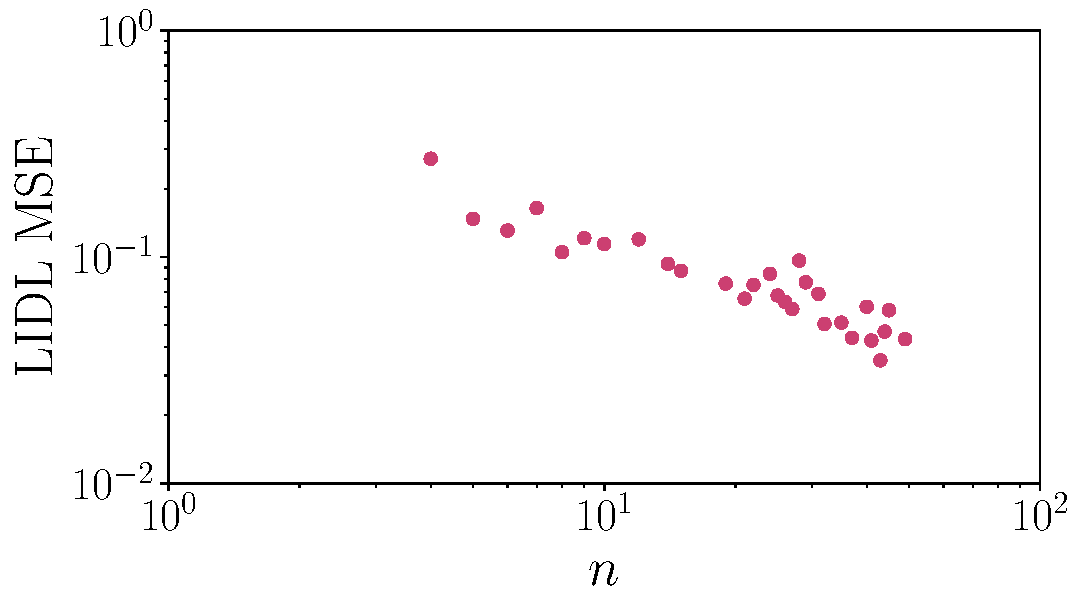
\includegraphics[width=0.4\textwidth]{images/mse-n-models.pdf}
    \caption{The dependence of mean-square error (MSE) on the number of models used in LIDL ($n$ from Algorithm\ref{alg:lidl}). We can observe monothonic decrease of the estimate error with the increase of $n$.}
    \label{fig:mse-n-models}
\end{figure}

\begin{figure}[h]
    \centering
    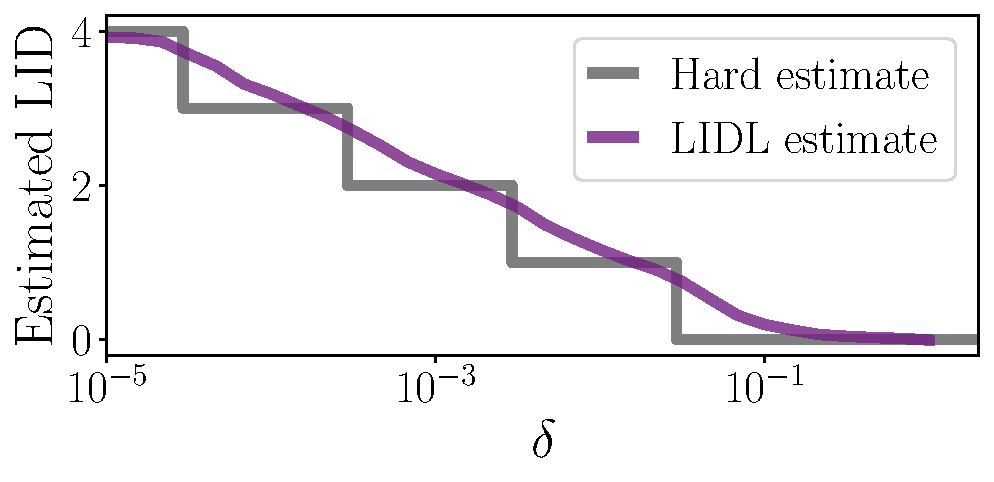
\includegraphics[width=0.4\textwidth]{images/step-delta-uniform.pdf}
    \caption{LIDL and hard estimate for different values of $\delta$ for 4-dimensional multiscale uniform distribution. We can see that LIDL ignores dimensions that are much smaller than $\delta$ even with imperfect density estimators.}
    \label{fig:step-delta-uniform}
\end{figure}




\begin{figure}[h]
\centering
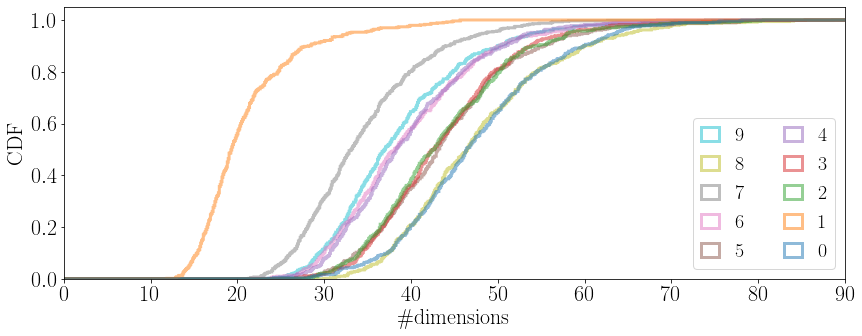
\includegraphics[width=0.9\textwidth]{images/mnist-cdf.png}
\caption{Empirical CDF of 5000 examples from MNIST dataset. Each line represents CDF for separate class in the dataset. Class number (which also is a represented digit in this case) can be found in the legend.}
\label{fig:mnist-cdf}
\end{figure}
\begin{figure}[h]
\centering
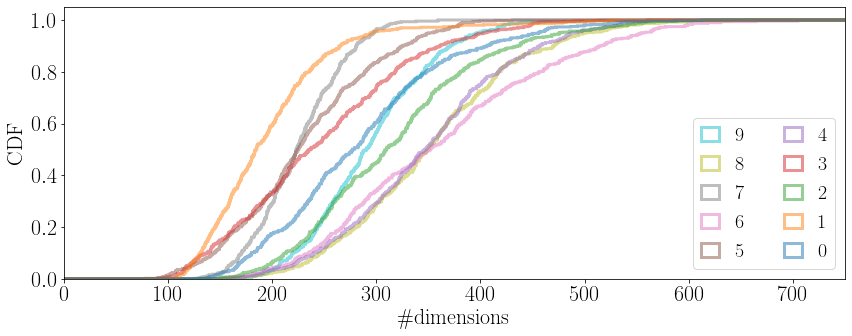
\includegraphics[width=0.9\textwidth]{images/fmnist-cdf.png}
\caption{Empirical CDF of 5000 examples from FMNIST dataset. Each line represents CDF for separate class in the dataset. Class number can be found in the legend.}
\label{fig:fmnist-cdf}
\end{figure}

\subsection{Image datasets}
\label{sec:details-image}
We present cumulative distribution function (CDF) for MNIST and FMNIST in Fig.~\ref{fig:mnist-cdf}~and~\ref{fig:fmnist-cdf}.  More samples from MNIST, FMNIST, Celeb-A sorted by their LID can be found in Fig.~\ref{fig:mnist-sort},~\ref{fig:fmnist-sort},~and~\ref{fig:celeba-sort}.


We can observe, that dimensionality estimates obtained from LIDL on MNIST are higher than those reported in \cite{pope2020intrinsic} or \cite{kleindessner2015dimensionality} and obviously depend on choosing the range of $\delta$s. We want to present some argument for our estimates:
\cite{cavallari2018unsupervised} used auto-encoder representation of MNIST as an input to SVN digit classifier and they achieved the best classification results for an auto-encoder with latent space size greater than 100. This means that we need more than 100 dimensions to encode an average MNIST digit to preserve all the information about it. Of course the compression with autoencoder is not ideal, but we can argue that true ID lies somewhere between.

\paragraph{Relation between examples for different range of $\delta$s}
We observed that for image dataset LID estimates for two disjoint sets of 4 $\delta$s have similar ranks (they on average differ between 10\%-15\%), and relations between points in each set (i.e. if LID estimate for $x_j$ is lower than LID estimate for $x_i$) are preserved in 80-90\% of cases. This of course depends strongly on $\delta$ range and the dataset.

\paragraph{LID estimate dependence on $\delta$ and effect of dequantization}


We present MNIST and FMNIST LID estimates (averaged per class) dependence on $\delta$ in Fig.~\ref{fig:mnist-delta-dependence}~and~\ref{fig:fmnist-delta-dependence}. Images present wide range of $\delta$s (from $10^{-4}$ to $10^{1}$) for original datasets and datasets with dequantization used after training. Black dashed line indicates a theoretical $\delta$, above which LIDL should not calculate dequantization dimensions into LIDL estimate. This is 10 times standard deviation of dequantization noise $\mathcal{U}(0,1/255)$. We can see that slightly above this threshold estimates for quantized and dequantized datasets aligh with each other. We can also observe, that for dequantized datasets and very small $\delta$ LID estimate is close to the dimensionality of the space, and for very big $\delta$s, LID estimates are close to 0 as expected.

\subsection{LID and model performance}
\label{sec:performance}
In this section, we show, that LID estimates are connected with model behavior on some benchmark datasets for autoencoder and classification deep neural networks.
Our result suggests, that the connection between LID and model performance is significant, so LIDL estimates can potentially be used in problems like semi-supervised learning, active learning, uncertainty estimation, and curriculum learning.

\paragraph{Reconstruction error vs LID for autoencoders}
\begin{figure}[h]
    \centering
    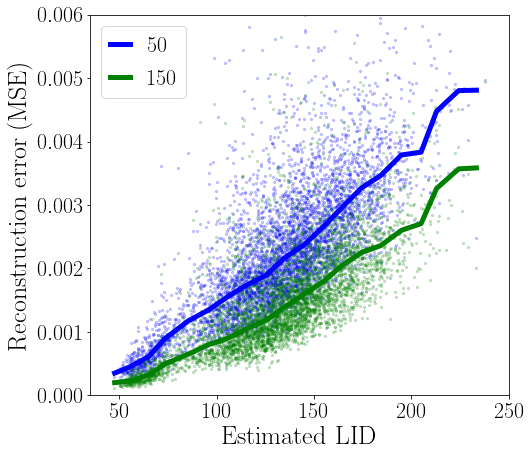
\includegraphics[width=0.45\textwidth]{images/LID-mse.png}
    \caption{LIDL estimates and VAE MSE scatterplot for a sample from MNIST dataset. Lines are running medians for those point clouds. Values in legend are VAE latent space size.}
    \label{fig:lid-mse}
\end{figure}

Results from the previous section led us to next experiment, where we wanted to investigate if the estimate from LIDL is correlated with reconstruction error for the image in VAE \citep{kingma2014auto}. We trained VAE on MNIST with latent space sizes 50 and 150, and observed that there is a high correlation (Pearsons $R > 0.7$ in both cases) between MSE and LID. We plotted LIDL estimates against MSE for 5K images in Fig.~ \ref{fig:lid-mse}. We can see an almost linear relationship between those quantities.

\paragraph{LID and classification accuracy}

We observed that classifiers can achieve better accuracy on data points with lower LID estimates. We trained neural networks on a subset of MNIST (300 images) and FMNIST (50K images) datasets and noticed a negative correlation of LID and an accuracy on a test set. Results are presented in Fig~\ref{fig:lid-accuracy}. What is more, we observed similar behavior inside a majority of classes (9 classes for MNIST, and 8 for FMNIST). 
\begin{figure}[h]
    \begin{subfigure}{.5\textwidth}
      \centering
      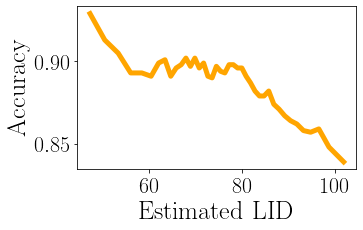
\includegraphics[width=0.6\linewidth]{images/accuracy-mnist.png}
    \end{subfigure}%
    \begin{subfigure}{.5
    \textwidth}
      \centering
      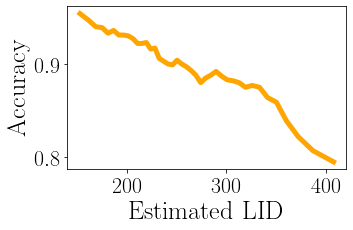
\includegraphics[width=0.6\linewidth]{images/accuracy-fmnist.png}
    \end{subfigure}
    \caption{Average classifier accuracy per LID value on MNIST(left) and FMNIST(right) datasets. We can see a very strong negative correlation between those values.}
    \label{fig:lid-accuracy}
\end{figure}



\begin{figure}[h]
\centering
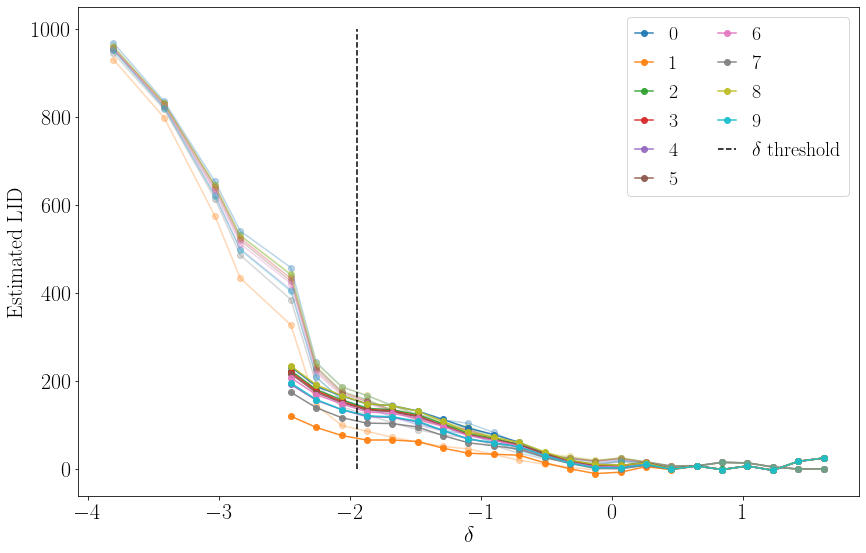
\includegraphics[width=0.99\textwidth]{images/quant-dequant-mnist.png}
\caption{MNIST average LID estimates for each class for quantized (strong color) and dequantized (faded colors) as a function of $\delta$.}
\label{fig:mnist-delta-dependence}
\end{figure}
\begin{figure}[h]
\centering
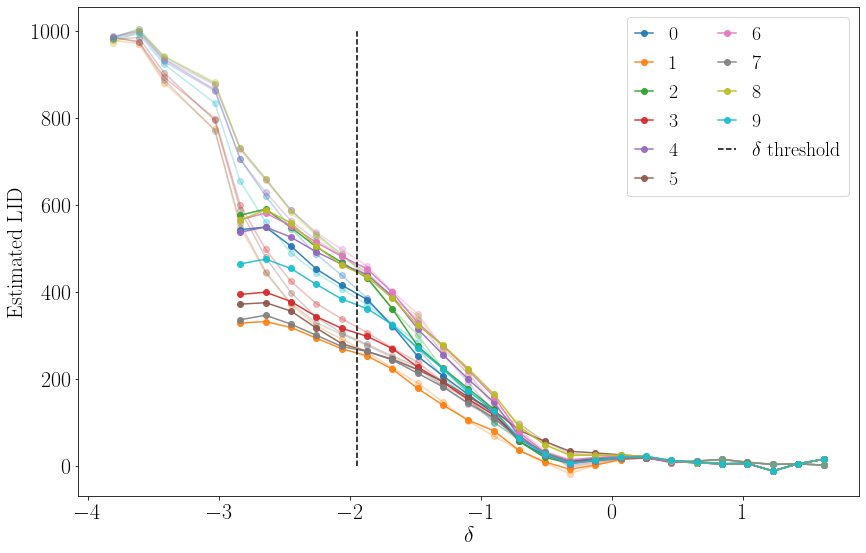
\includegraphics[width=0.99\textwidth]{images/quant-dequant-fmnist.png}
\caption{FMNIST average LID estimates for each class for quantized (strong color) and dequantized (faded colors) as a function of $\delta$.}
\label{fig:fmnist-delta-dependence}
\end{figure}

\begin{figure}[t]
\centering
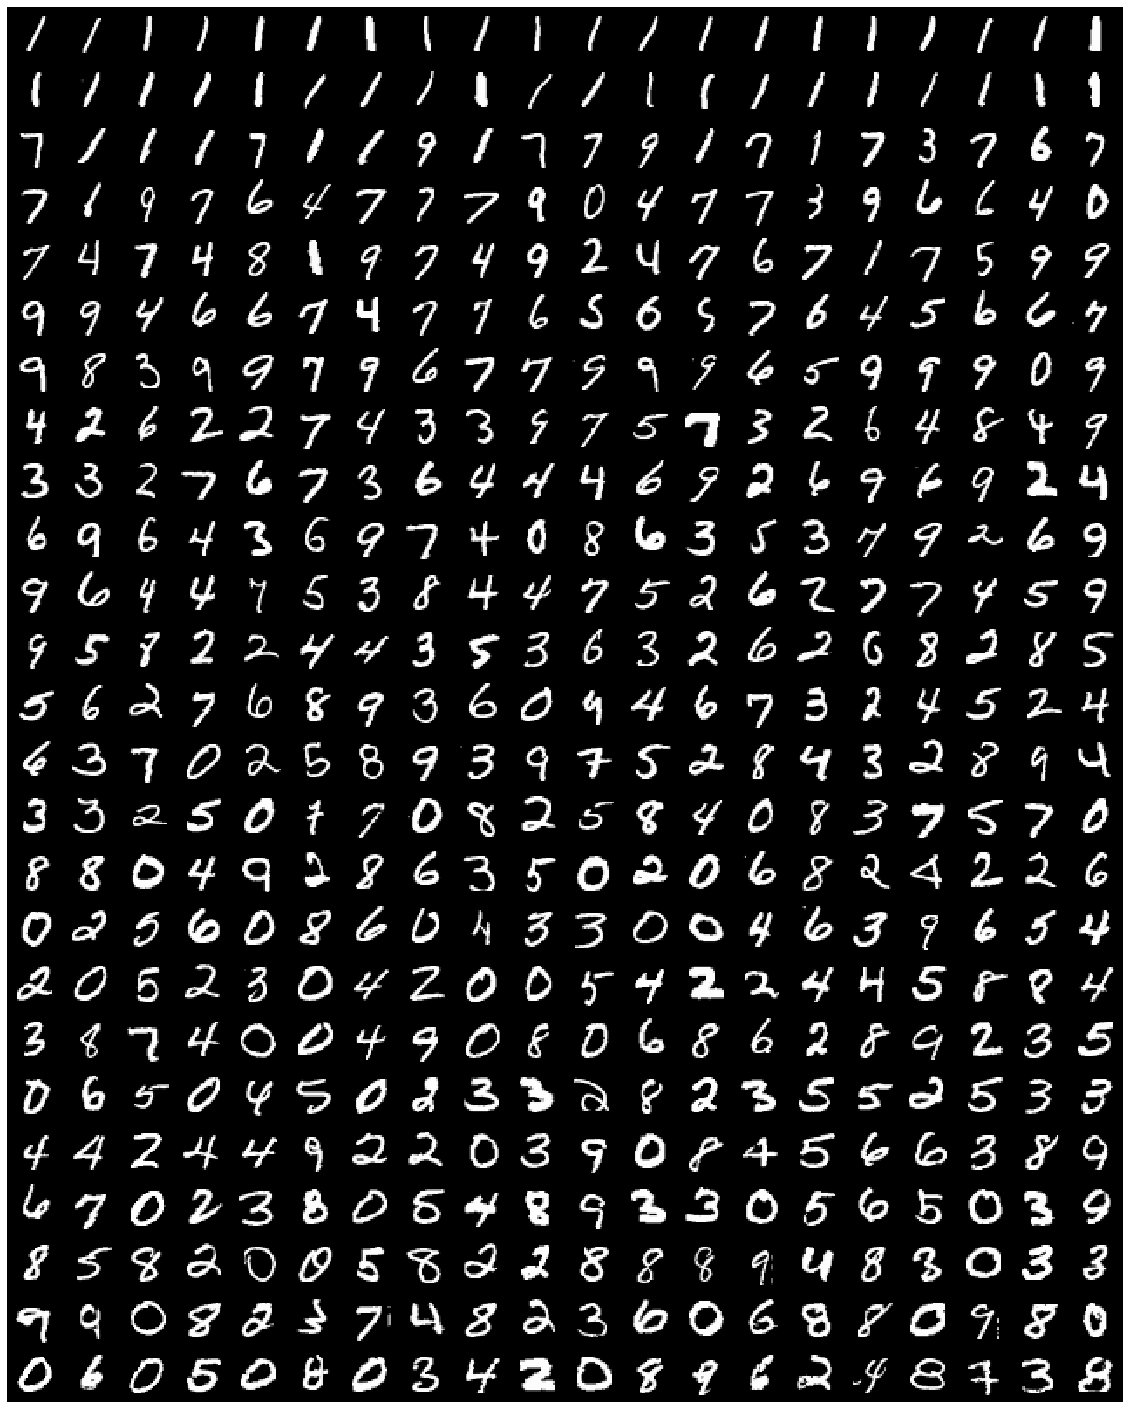
\includegraphics[width=0.95\textwidth]{images/mnist-sorted.png}
\caption{Samples from MNIST sorted by their LID estimates.}
\label{fig:mnist-sort}
\end{figure}
\begin{figure}[t]
\centering
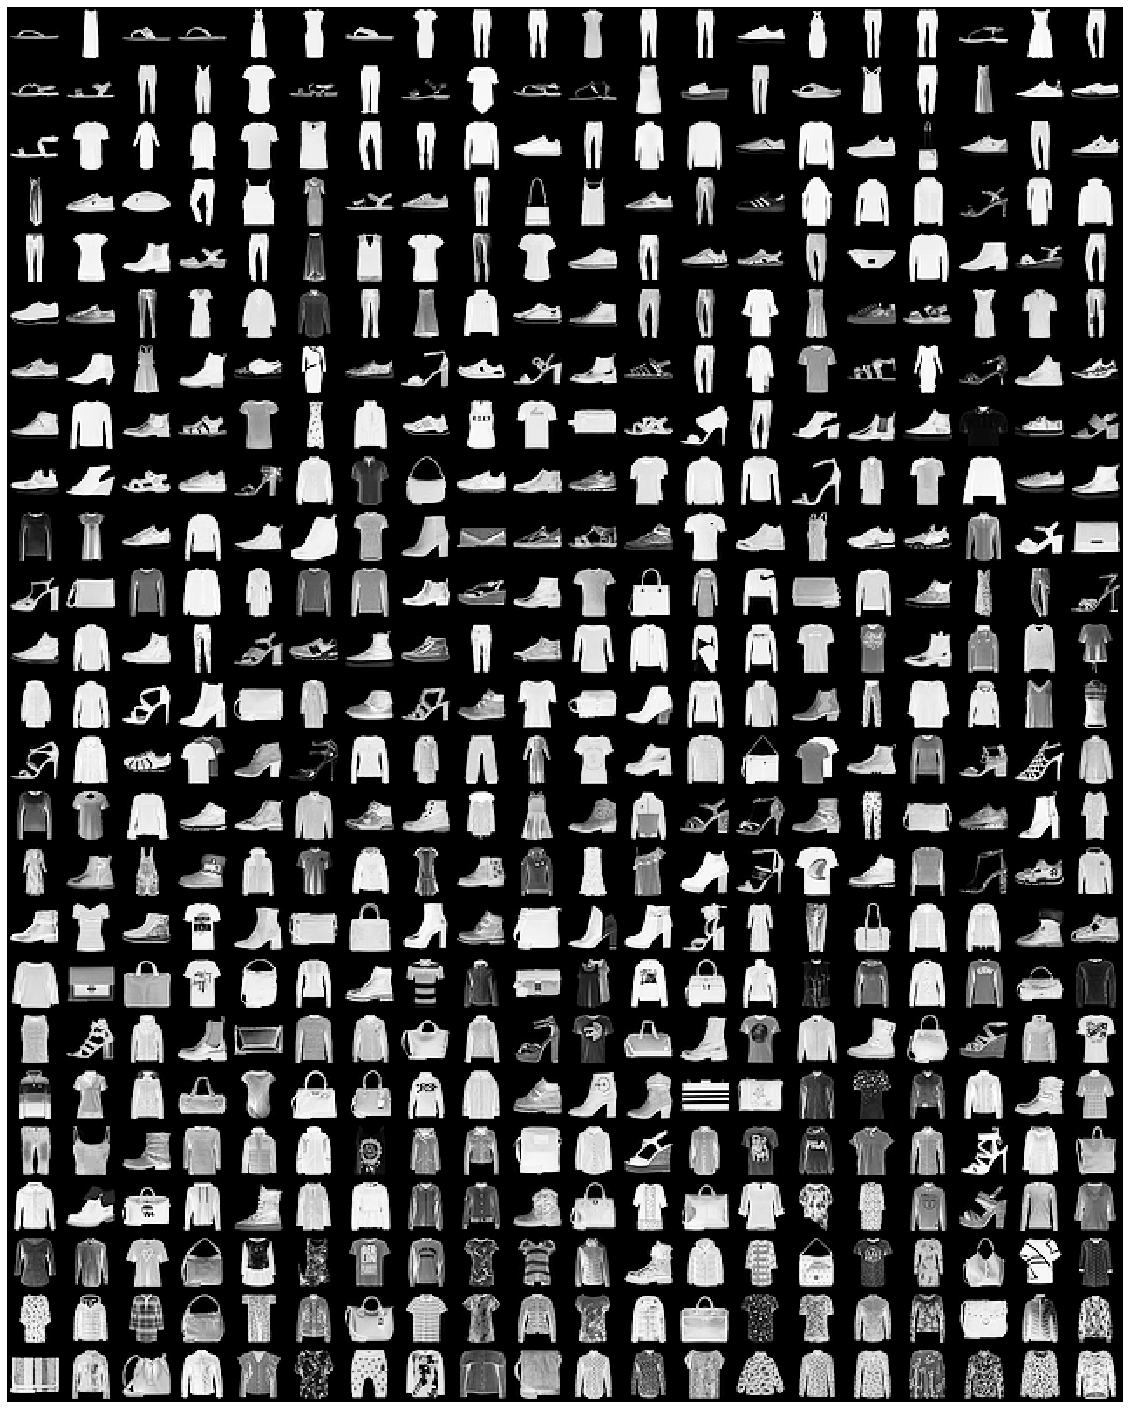
\includegraphics[width=0.95\textwidth]{images/fmnist-sorted.png}
\caption{Samples from FMNIST sorted by their LID estimates.}
\label{fig:fmnist-sort}
\end{figure}
\begin{figure}[t]
\centering
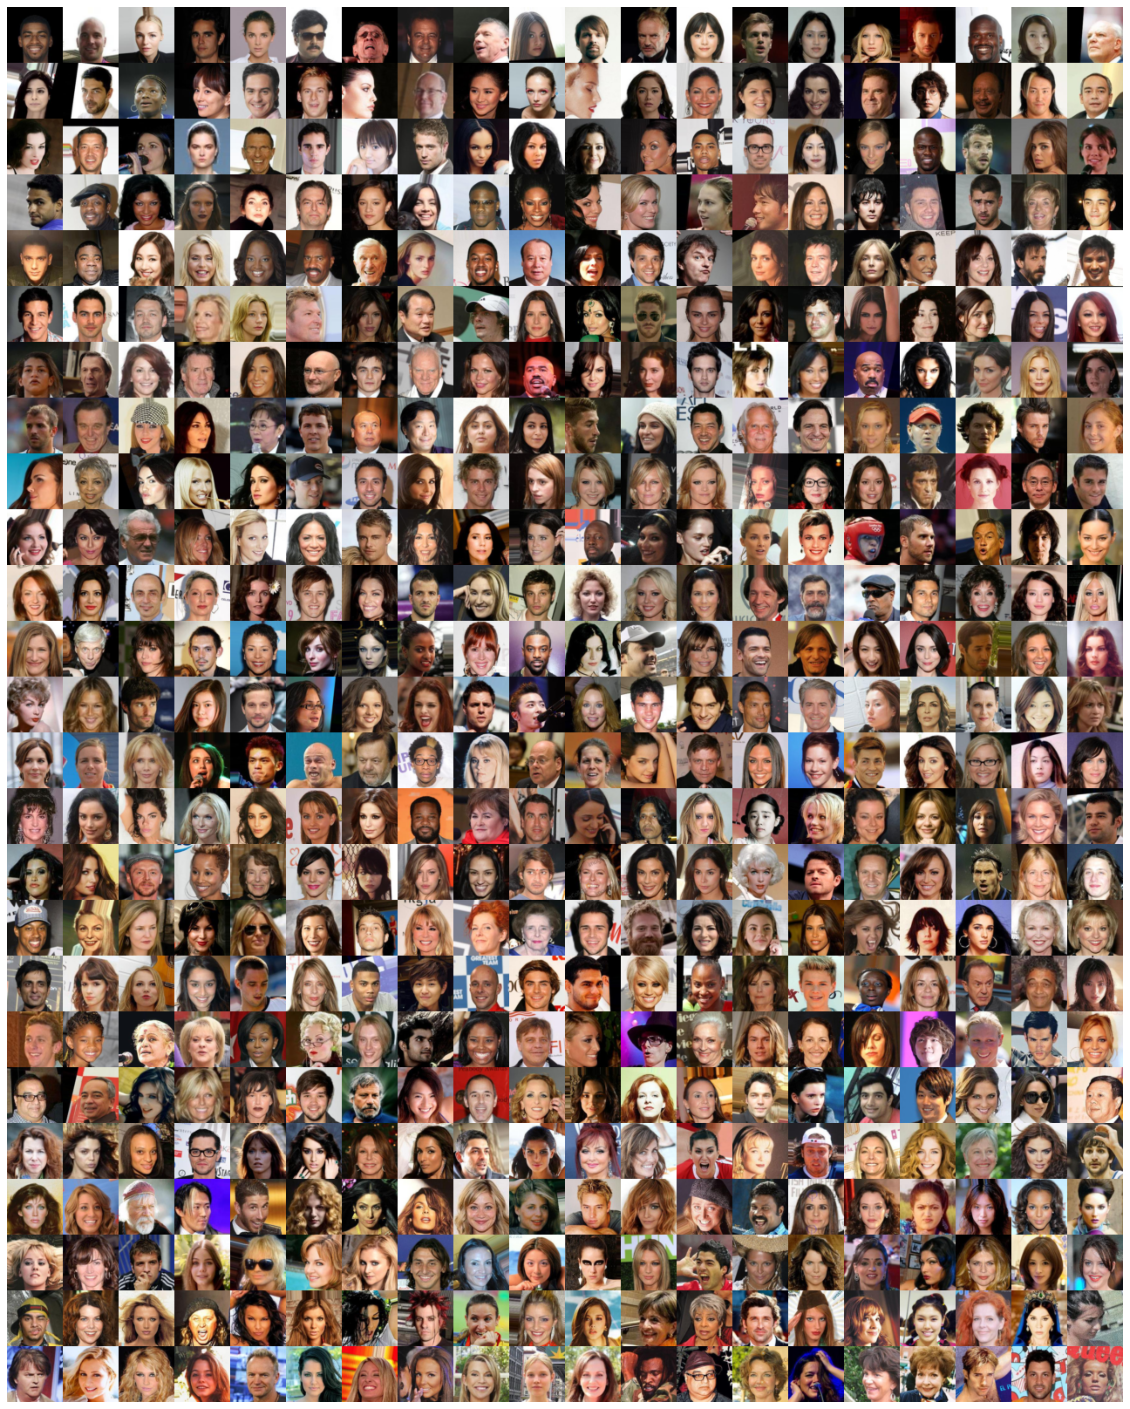
\includegraphics[width=0.95\textwidth]{images/celeba-sorted.png}
\caption{Samples from Celeb-A sorted by their LID estimates.}
\label{fig:celeba-sort}
\end{figure}


